\subsubsection{Syntax Trees}

Now that the parser has been generated by gt it is ready to be used. A useful feature
of gt is being able to generate visual syntax trees. The example will show the 
syntax tree that is generated by the above grammar. Figure 2.1 is an example of a 
that was generated by gt's gviz function. \\ \\

\begin{figure}[h!]
  \centering
  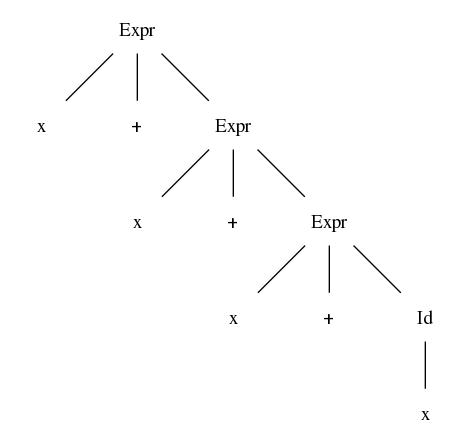
\includegraphics[width=3in]{./examples/bnf/simple/simple.png}
  \caption{Syntax Tree for\\ \textit{x + x + x + x}}
\end{figure}




